% Page no - 11
\subsection{Viola's Framework}
\par
Almost all the state of the art face detection systems are developed upon Viola’s Framework, based on AdaBoost and Haar features. The philosophy of AdaBoost is that if it is hard to find a good (strong) classifier directly, we can construct a lot of poor quality ones (weak classifier) $h_m (x) ,m = 1, . . . , M$ and use the combination of them to form a strong classifier [27]:

\begin{equation}
    H_M(x) = \frac{\sum_m{a_mh_m(x)}}{\sum_M{a_m}}
\end{equation}

where $a_m ≥ 0$ are the combining coefficients. In the discrete version $h_m(x)$ gives either $−1$
or $1$ whereas in the real version, the output can be a real number. Because we need a lot of weak classifiers, $h_m(x)$ is normally chose to have a simple form (so it is easy to construct). In Viola and Jones’s work, they use threshold classifiers, each of which works on one feature selected from an over-complete set of Haar wavelet-like features. We’ll first introduce Haar Wavelet, then give the iterative algorithm of AdaBoost.

\subsubsection{Haar Wavelet}

\par
Wavelet analysis is a tool for signal processing which can perform local analysis. It is useful in face detection because we want to focus on a localized area of the image and find whether it contains a face. Haar wavelet is the first known wavelet, and probably the simplest one. A one-dimensional Haar wavelet function is just a step function, as shown in Fig.2.5(a).

\par
In image processing, two-dimensional wavelets are used which look like the ones in Fig.2.5(b). The functions in Fig.2.5(b) don’t satisfy some conditions of a wavelet (because we don’t need those in our application), so strictly speaking they are ``Haar-like features''. An important property of Haar wavelet-like features is that they can be computed efficiently using an integral image. The integral image $II(x, y)$ of image $I(x, y)$ is
defined by:

\begin{equation}
    II(x, y) = \sum_{x' < x, y' < y}{I(x' , x')}
\end{equation}

\newpage
% Page no - 12
\begin{figure}[h!]
    \centering
    \begin{subfigure}{0.25\textwidth}
      \centering
      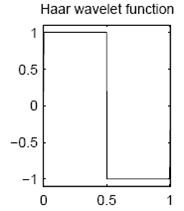
\includegraphics{img/25_1.png}
      \caption{1-dimensional Haar Wavelet function}
      \label{fig:25_sub1}
    \end{subfigure}%
    \begin{subfigure}{0.25\textwidth}
      \centering
      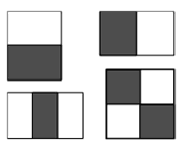
\includegraphics{img/25_2.png}
      \caption{Four types of 2-d Haar wavelet-like features}
      \label{fig:25_sub2}
    \end{subfigure}
    \caption{Haar Wavelet and Haar features}
    \label{fig:25}
\end{figure}

\par
This can be computed in one pass over the original image as follows:

\begin{equation}
    S(x, y) = S(x, y - 1) + I(x, y)
\end{equation}

where $S(x, y)$ is the cumulative sum of the $x$th row. Apparently $S(x, 0) = 0$ and $II(0, y) = 0$. Any rectangular sum in an image can be expressed in terms of its integral image as illustrated in \ref{fig:29}

\par
The sum of the pixels within rectangle $D$ in \ref{fig:29} can be computed using the integral image value on points $a, b, c, d$ as follows:

\begin{equation}
    II(x2, y2) = \sum_{x<x2, y<y2}{I(x, y)} = A + B + C + D
\end{equation}

\begin{equation}
    II(x2, y1) = \sum_{x<x2, y<y1}{I(x, y)} = A + C
\end{equation}

\begin{equation}
    II(x1, y2) = \sum_{x<x1, y<y2}{I(x, y)} = A + B
\end{equation}

\begin{equation}
    II(x1, y1) = \sum_{x<x2, y<y2}{I(x, y)} = A
\end{equation}

\begin{equation}
    D = II(x2, y2) + II(x1, y1) - II(x2, y1) - II(x1, y2)
\end{equation}

\newpage